The off-the-shelf knn classfier used was the one implemented in the R package \emph{'class'} written by Brian Ripley. The key settings used for this classification were - 
\begin{itemize}
		\item Preprocessing - Simple Scaling with Binning(same as classifier 3)
		\item Proximity Metric - (internal)
		\item Voting - (internal)
\end{itemize}
The classifier performed significantly better than any of our classifiers. The AUC peaked at $k=29$. The ROC curve at $k=29$ also rose sharply and then saturated at $FPR=0.6$. The AUC was greater than either of out classfiers. Finally the accuracy also rose quickly with threshold and reached a saturation at $0.8$.\\

\begin{figure}[h]
	\label{fig:classifier2_auc}
	\caption{Plot of Area Under the Roc curve for different values of k for Income dataset for off-the-shelf-knn. Maxima is achieved at k = 29}
	\centering
	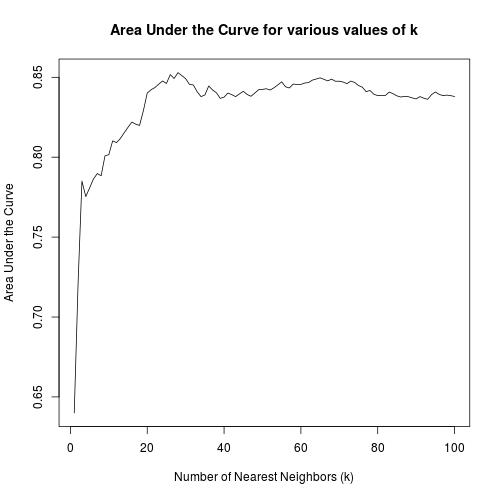
\includegraphics[width=0.3\textwidth]{images/native-knn/auc.jpg}
\end{figure}	
\begin{figure}
	\label{fig:classifier2_roc}
	\caption{ROC curves for different values of k for Income Classifier 2}
	\centering
	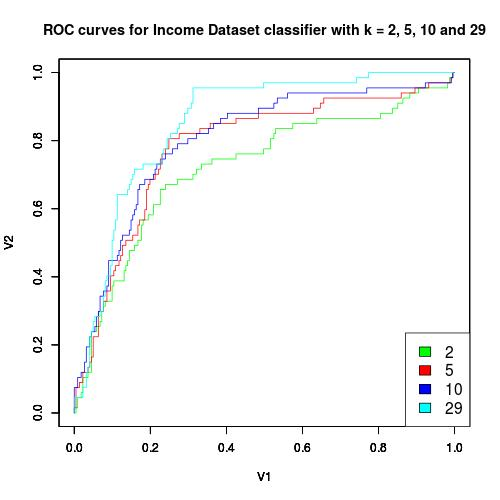
\includegraphics[width=0.3\textwidth]{images/native-knn/roc.jpg}
\end{figure}
\begin{figure}
	\label{fig:classifier2_accuracy}
	\caption{Plot of Accuracy Vs Threshold Values for k = 29}
	\centering
	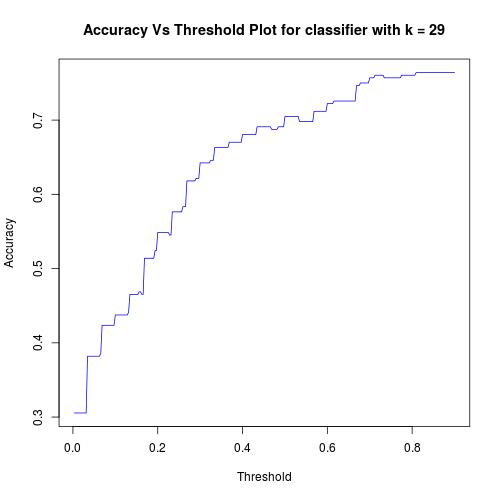
\includegraphics[width=0.3\textwidth]{images/native-knn/accuracy.jpg}
\end{figure}

